La envoltura convexa de un conjunto de puntos es el polígono convexo más pequeño que rodea todo el conjunto y tiene una serie de aplicaciones prácticas. Un método eficiente que se usa a menudo en los desafíos es el escaneo de Graham, que requiere una clasificación por ángulo. Esto no es tan fácil como parece al principio, ya que calcular los ángulos reales es costoso e introduce problemas de error numérico. Un algoritmo más simple pero igualmente eficiente se debe a Andrew, y requiere solo una ordenación por $X$ para un barrido de línea aunque el artículo original de Andrew ordena por $Y$ y tiene algunas optimizaciones que no discutiré aquí.

El algoritmo de Andrew divide la envoltura convexa en dos partes, la envoltura superior y el inferior. Por lo general, estos se encuentran en los extremos, pero si más de un punto tiene una coordenada X mínima (o máxima), entonces se unen mediante un segmento de línea vertical. Describiremos cómo construir la envoltura superior; la envoltura inferior se puede construir de manera similar y, de hecho, se puede construir en el mismo bucle.

Para construir el casco superior, comenzamos con el punto con la coordenada $X$ mínima, rompiendo los lazos tomando la coordenada $Y$ más grande. Después de esto, los puntos se agregan en el orden de la coordenada $X$ (siempre tomando el valor Y más grande cuando varios puntos tienen el mismo valor $X$). Por supuesto, a veces esto hará que el casco se vuelva cóncavo en lugar de convexo:


% TODO: \usepackage{graphicx} required
\begin{figure}[h!]
	\centering
	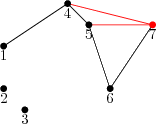
\includegraphics[width=0.2\linewidth]{img/uhull}
	\label{fig:uhull}
\end{figure}


El camino negro muestra el casco actual. Después de agregar el punto 7, verificamos si el último triángulo (5, 6, 7) es convexo. En este caso no lo es, por lo que eliminamos el penúltimo punto, es decir, el 6. El proceso se repite hasta encontrar un triángulo convexo. En este caso también examinamos (4, 5, 7) y eliminamos 5 antes de examinar (1, 4, 7) y encontrar que es convexo, antes de pasar al siguiente punto. Este es esencialmente el mismo procedimiento que se usa en la exploración de Graham, pero procediendo en el orden de la coordenada $X$ en lugar del orden del ángulo formado con el punto de partida. A primera vista, puede parecer que este proceso es O($N^2$) debido al bucle interno de retroceso, pero dado que ningún punto se puede eliminar más de una vez, en realidad es O($N$). El algoritmo general es O($N \log N$), porque los puntos deben ordenarse inicialmente por la coordenada $X$.